%----------------------------------------------------------------------------------------
%    PACKAGES AND THEMES
%----------------------------------------------------------------------------------------

\documentclass[aspectratio=169,xcolor=dvipsnames]{beamer}
\setbeameroption{show notes} %TODO: Thomas a enlever avant la presentation
\usetheme{SimplePlus}

\useoutertheme{miniframes}  % Adds horizontal navigation dots at the top for subsections

\usecolortheme{} 

\setbeamercolor{block title}{bg=structure,fg=white}  % Navy blue background for block titles
\setbeamercolor{block body}{bg=structure!10,fg=black}  % Light navy tint for block body

\definecolor{darkwine}{RGB}{128,0,32}  % Dark red wine
\newenvironment{errorblock}[1]{%
\begingroup%
\setbeamercolor{block title}{bg=darkwine,fg=white}%
\setbeamercolor{block body}{bg=structure!05,fg=black}%  % Very close to white background
\begin{block}{#1}%
}{\end{block}\endgroup}

\usepackage{comment}
\usepackage{hyperref}
\usepackage{graphicx} % Allows including images
\usepackage{booktabs} % Allows the use of \toprule, \midrule and \bottomrule in tables
\usepackage{array} % Allows >{\centering\arraybackslash} in tabular
\usepackage[utf8]{inputenc} % Handle Unicode characters
\usepackage[T1]{fontenc} % Better font encoding
\usepackage{amsmath,amssymb} % Math symbols

% Define hyphenation command
\newcommand{\hyp}{-}

%----------------------------------------------------------------------------------------
%    TITLE PAGE
%----------------------------------------------------------------------------------------

\title{Diffusion Generative Flow Samplers: Improving Learning Signals Through Partial Trajectory Optimization}

\subtitle{Dinghuai Zhang*, Ricky T. Q. Chen, Cheng-Hao Liu, Aaron Courville \& Yoshua Bengio}
\author{Thomas Mousseau} 

% \institute
% {
%     Department of Computer Science and Information Engineering \\
%     National Taiwan University % Your institution for the title page
% }
\date{\today} % Date, can be changed to a custom date

%----------------------------------------------------------------------------------------
%    PRESENTATION SLIDES
%----------------------------------------------------------------------------------------

\begin{document}

\begin{frame}
    % Print the title page as the first slide
    \vspace*{-2cm}
    \titlepage
\end{frame}

\begin{frame}{Overview}
    % Throughout your presentation, if you choose to use \section{} and \subsection{} commands, these will automatically be printed on this slide as an overview of your presentation
    \tableofcontents
\end{frame}

%------------------------------------------------

\section{Introduction}

\subsection{Problem Statement}

\begin{frame}[t]{Generative Modeling}
\scriptsize
\begin{block}{Task}
    Sample from a complex (high-dimensional and multimodal) distribution $D$.
\end{block}

$D$ can be given under the form of:

\begin{columns}[t]
\begin{column}{0.48\textwidth}
\begin{itemize}\itemsep2pt
    \item A dataset of samples $\{x_i\}_{i=1}^N \sim D$ (e.g., images, text, audio)
    \begin{figure}
        \centering
        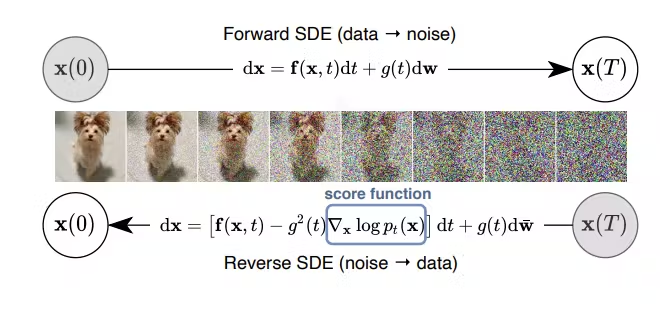
\includegraphics[width=0.9\textwidth]{figures/score_diffusion.png}
    \end{figure}
\end{itemize}
\end{column}
\begin{column}{0.48\textwidth}
\begin{itemize}\itemsep2pt
    \item An unnormalized density $\mu(x)$ where $D$ has density $\pi(x) \propto \mu(x)$ (e.g., 
    energy-based models, physics/chemistry)
    \begin{figure}
        \centering
        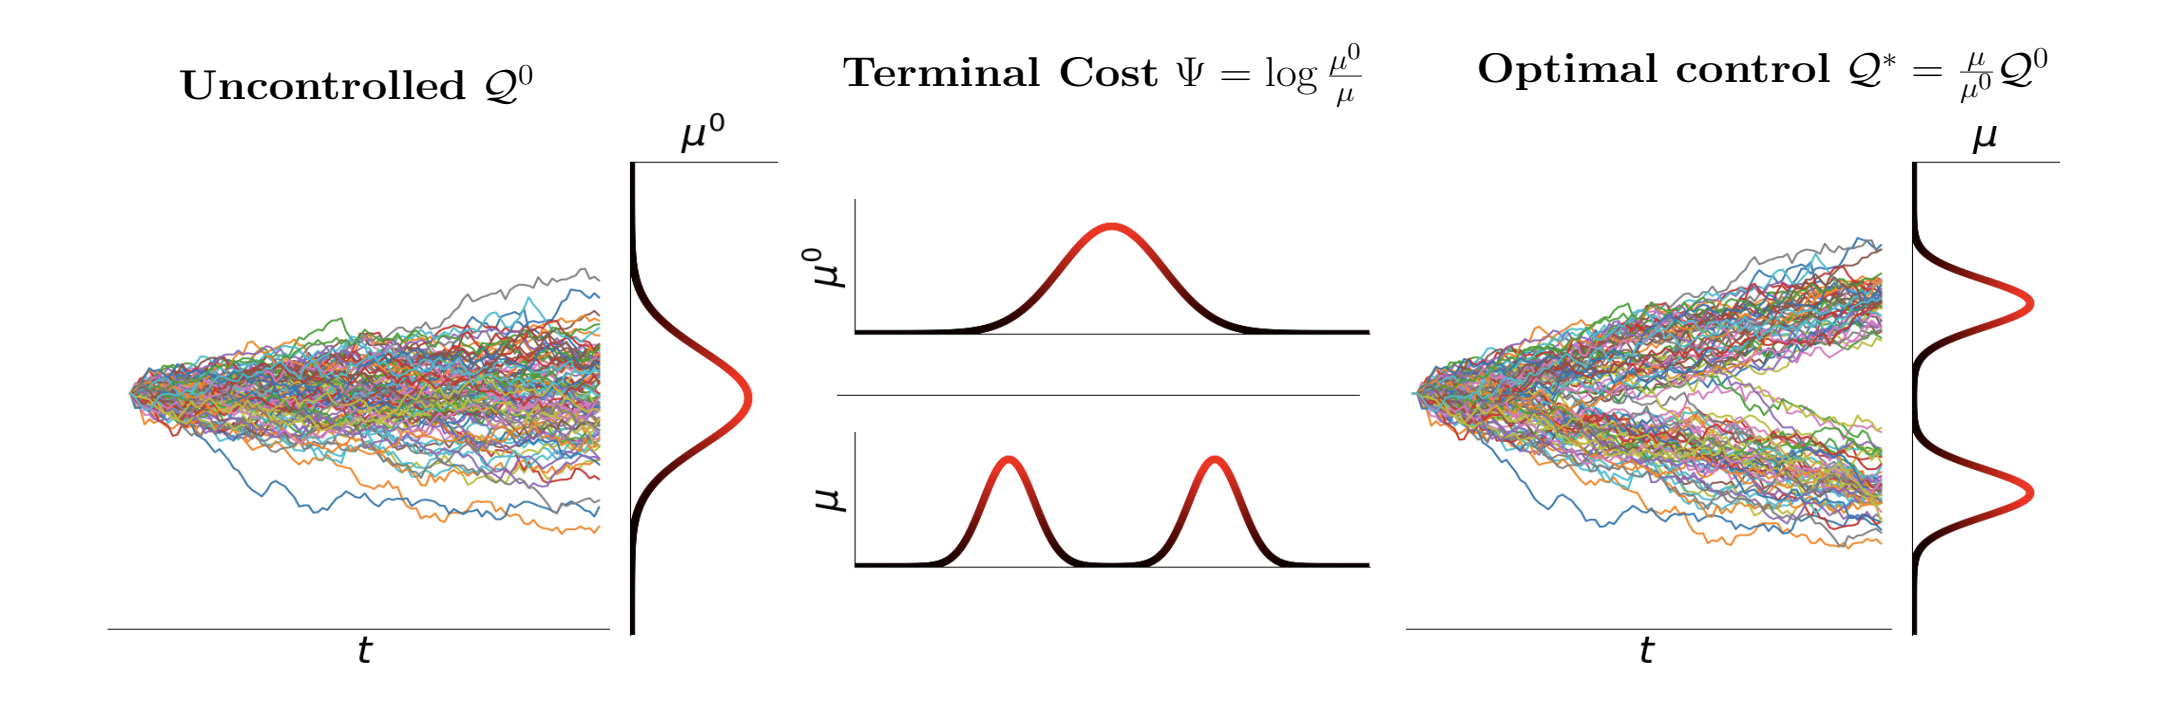
\includegraphics[width=0.9\textwidth]{figures/unconctrolled.png}
    \end{figure}
\end{itemize}
\end{column}
\end{columns}

\end{frame}

\begin{frame}[t]{Sampling from Unnormalized Densities}
\footnotesize
\textbf{Context.} Sample from a $D$-dimensional target with unnormalized density $\mu(x)$ where $\mathbb R^D \to \mathbb R^+$.
\[
\pi(x)=\frac{\mu(x)}{Z},\qquad Z=\int_{\mathbb R^D}\mu(x)\,dx\ \text{(unknown)}.
\]
We assume we can evaluate $\mu(x)$, but we have no samples from $\pi$ and do not know $Z$.

\vspace{0.1cm}

\medskip
\textbf{Goal.} We seek a \emph{sampler} (similar to MCMC/VI) that produces calibrated samples and, ideally, estimates $Z$ \emph{without} any dataset from $\pi$.

\vspace{0.3cm}

\begin{block}{\scriptsize Chemistry (molecule conformers).} \scriptsize Different 3D conformations have a formation energy from force-field terms (bonds, angles, dihedrals, nonbonded). A low energy means a higher probability of being sampled. A well-calibrated sampler is needed to draw conformers in proportion to these probabilities, which is important in binding-pose ranking, free-energy estimation and generating diverse realistic 3D conformers for screening.
\end{block}

\end{frame}

\begin{frame}[t]{Diffusion Generative Flow Samplers}
\footnotesize
\textbf{Idea.} We will \emph{reframe sampling} from an unnormalized target $\pi(x)\propto \mu(x)$ as a \emph{stochastic optimal control (SOC)} problem. This means learning a control function that steers a diffusion process so its \emph{terminal marginal} matches $\pi$.

\medskip
\textbf{Why this helps.}
\begin{itemize}\itemsep2pt
  \item Gives a \emph{path-space} training objective/metric: a KL on trajectories $\mathrm{KL}(Q\,\|\,P)$ where $P$ is the reference paths reweighted by $\mu(x_T)$.
  \item The \emph{partition function $Z$ cancels} inside this objective, so we can train using only $\mu$ (and optionally $\nabla\log\mu$).
  \item Lets us optimize \emph{without samples from $\pi$} and still measure closeness to the true normalized endpoint.
\end{itemize}

\medskip
\textbf{Caveat (sets up DGFS).} This path-KL places supervision \emph{only at the terminal time} $\Rightarrow$ poor \emph{credit assignment} and high-variance gradients.

\medskip
\textbf{DGFS fix (preview).} Inject \emph{intermediate} learning signals via a GFlowNet-inspired \emph{learned flow} and \emph{subtrajectory balance}, enabling partial-trajectory training and more stable learning.
\end{frame}

\begin{frame}[t]{Diffusion Generative Flow Samplers v2}

    Minimizing the running and terminal costs between the optimal controlled process and the uncontrolled reference process.

\begin{figure}
    \centering
    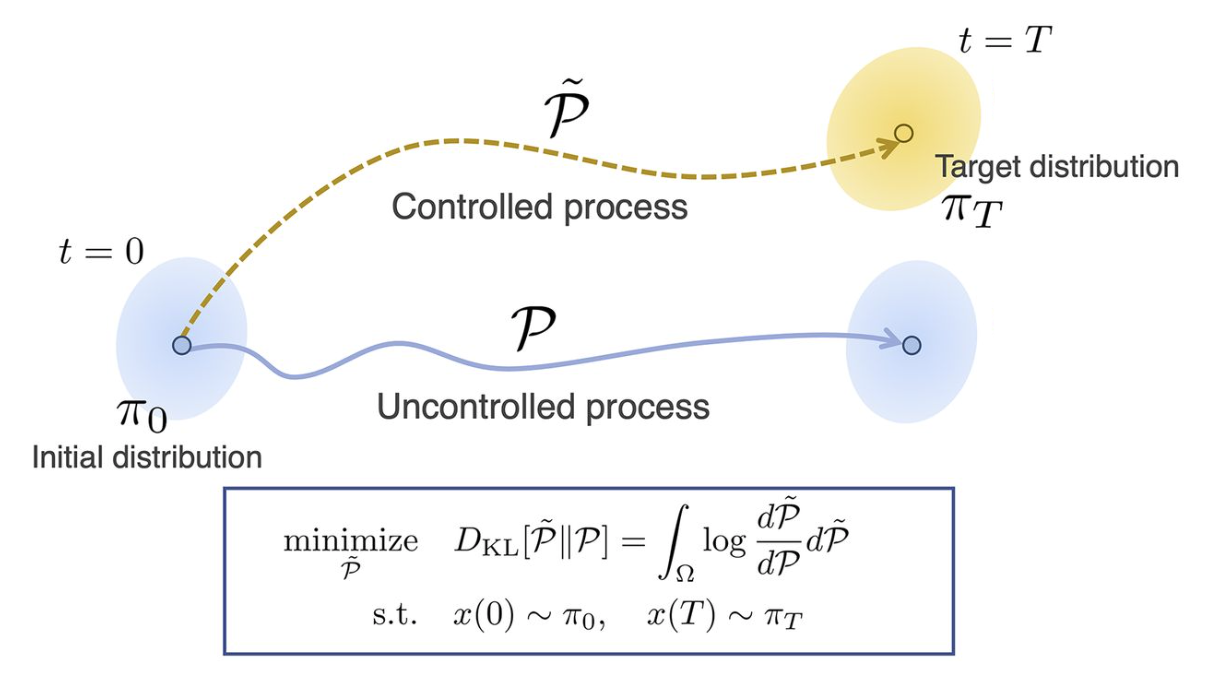
\includegraphics[width=0.6\textwidth]{figures/image.png}
\end{figure}

\note{refaire cette illustration avec le controlled, uncontrolled et target (optimal controlled) processus }

\end{frame}


\subsection{Stochastic Optimal Control}

\begin{frame}[t]{Controlled and Reference Processes}
\scriptsize
\textbf{Controlled forward transition (learned drift).}
\[
P_F(x_{n+1}\mid x_n)\;=\;\mathcal N\!\big(x_{n+1};\;x_n + h\,f_\theta(x_n,n),\;h\sigma^2 I\big)
\]
\textbf{Controlled process.}
\[
Q(x_{0:N})\;=\;p^{\text{ref}}_0(x_0)\;\prod_{n=0}^{N-1} P_F(x_{n+1}\mid x_n)
\]

\medskip
\textbf{Uncontrolled/Reference forward transition (zero drift).}
\[
P_F^{\text{ref}}(x_{n+1}\mid x_n)\;=\;\mathcal N\!\big(x_{n+1};\;x_n,\;h\sigma^2 I\big)
\]
\textbf{Uncontrolled/Reference process and marginals.}
\[
Q^{\text{ref}}(x_{0:N})\;=\;p^{\text{ref}}_0(x_0)\;\prod_{n=0}^{N-1} P_F^{\text{ref}}(x_{n+1}\mid x_n),
\]

\[
p^{\text{ref}}_n(x) = \mathcal{N}\left( x; \mu_0, \Sigma_0 + n h \sigma^2 I \right), \;\text{is closed form.}
\]

\medskip
\textbf{Goal.} Learn $f$ so that the terminal marginal $Q(x_N)$ matches $\pi(x)=\mu(x)/Z$ (no data, $Z$ unknown.).

\note{Why closed form for uncontrolled but not controlled? The uncontrolled reference process has no drift, so each transition is a simple Gaussian convolution, leading to Gaussian marginals with closed-form means and variances $(e.g., p^{ref}_n(x) = N(x; mu_0, cov_0 + n h \sigma^2 I))$. The controlled process includes a learned drift $f(x_n, n)$, which makes transitions non-Gaussian and dependent on $f$, preventing a closed-form marginal expression without solving the integral numerically or via simulation.


\textcolor{red}{je dois refaire cette slide, on ne voit meme comment xn est sample (par rapport a la SDE) et aussi d'ou sort sigma mu et la closed form expliquer et c'est une convolution de gaussienne}
}

\end{frame}



% \begin{frame}[t]{Target Path Measure via IS (Part 2)}
% \footnotesize

% \textbf{What Each Term Does.}
% \begin{itemize}\itemsep2pt
%   \item \( Q^{\text{ref}}(x_{0:N}) \): The proposal path measure—provides the base trajectories (e.g., uncontrolled diffusion). It's the "easy" distribution we sample from.
%   \item \( \pi(x_N) \): The target terminal density (normalized). It steers the paths toward high-probability endpoints under the true distribution.
%   \item \( p^{\text{ref}}_N(x_N) \): The reference terminal marginal (known, e.g., Gaussian). It normalizes the weight so the reweighted measure integrates to 1 and corrects for the proposal's bias at the endpoint.
% \end{itemize}

% \textbf{Why This Achieves the Goal.} The weight \( w(x_{0:N}) \) adjusts the path probabilities so that trajectories ending in regions with high \( \mu(x_N) \) are favored, while those in low-\( \mu \) regions are penalized. This "importance resamples" the paths to match the target terminal distribution, without needing samples from \( \pi \).

% \textbf{Connection to Girsanov Theorem.} This reweighting is formalized by the **Girsanov theorem** in stochastic calculus, which allows changing the drift of a diffusion process by reweighting the path measure with an exponential martingale. Here, the weight \( \frac{\pi(x_N)}{p^{\text{ref}}_N(x_N)} \) corresponds to the Radon-Nikodym derivative that shifts the process from the reference (zero-drift) to one with the desired terminal behavior. It's not just importance sampling—it's a rigorous change-of-measure for continuous-time processes, ensuring the reweighted paths are absolutely continuous and the terminal marginal is exact.

% \end{frame}

% --- Slide 2 ---
\begin{frame}[t]{Path space KL objective}
\scriptsize
% \textbf{Elementary identity: P(A,B) = P(A$\mid$B) P(B)}
% \[
% P(x_{0:N}) = P(x_{0:N-1} | x_N) P(x_N).
% \]

% \textbf{Reference bridge decomposition.}
% \[
% Q^{\text{ref}}(x_{0:N}) \;=\; Q^{\text{ref}}(x_{0:N-1}\mid x_N)\; p_N^{\text{ref}}(x_N),
% \qquad p_N^{\text{ref}}(x_N)=\!\int Q^{\text{ref}}(x_{0:N})\,dx_{0:N-1}.
% \]

\textbf{Target path measure via terminal reweighting.}
\[
P(x_{0:N}) \;\propto\; Q^{\text{ref}}(x_{0:N-1} | x_N) \mu(x_N) \;\propto\ Q^{\text{ref}}(x_{0:N})\,\frac{\mu(x_N)}{p^{\text{ref}}_N(x_N)}
\qquad\Longrightarrow\qquad P(x_N)\propto\mu(x_N).
\]

\textbf{KL decomposition.}
\[
\mathrm{KL}(Q\|P)
=\mathbb E_{Q}\!\left[\log\frac{Q}{P}\right]
=\mathbb E_{Q}\!\left[\log\frac{Q}{Q^{\text{ref}}}\right]
+\mathbb E_{Q}\!\left[\log\frac{p^{\text{ref}}_N(x_N)}{\mu(x_N)}\right] + \log Z.
\]


\medskip
\textbf{Running control cost (Gaussian mean-shift) Girsanov theorem.}
\[
\mathbb E_{Q}\!\left[\log\frac{Q}{Q^{\text{ref}}}\right]
=\mathbb E_Q \sum_{n=0}^{N-1}\frac{h}{2\sigma^2}\,\|f_\theta(x_n,n)\|^2.
\]

\textbf{Terminal cost.}
\[
\mathbb E_{Q}\!\left[\log\frac{p^{\text{ref}}_N(x_N)}{\mu(x_N)}\right]
=\mathbb E_Q\!\big[\log p^{\text{ref}}_N(x_N)-\log \mu(x_N)\big]
\]

\note{ \textcolor{red}{Je devrais avoir une slide complete a explier d'ou vient le foward target process $P$ parce que c'est le coeur de mon algorithme} }
\end{frame}

\begin{frame}[t]{Target Path Measure via Importance Sampling}
\footnotesize

\textbf{Importance Sampling Basics.} Importance sampling is a technique to estimate expectations under a hard-to-sample target distribution \( P \) using samples from an easy-to-sample proposal distribution \( Q \). The key formula is:
\[
\mathbb{E}_{x \sim Q} \left[ f(x) \cdot w(x) \right] = \mathbb{E}_{x \sim P} [f(x)],
\]
where the \textcolor{red}{\emph{importance weight} \( w(x) = \frac{P(x)}{Q(x)} \)} corrects the samples from \( Q \) to behave as if they were from \( P \).

\textbf{Intuition.} \( Q \) provides "biased" samples; \( w(x) \) upweights samples that are likely under \( P \) and downweights those that aren't, effectively resampling from \( P \) without directly sampling it.

\textbf{Application to Path Measures.} In our case, the "samples" are entire trajectories \( x_{0:N} \), and we want the path measure \( P \) to have the correct terminal marginal \( \pi(x_N) \propto \mu(x_N) \). We use the reference path measure \( Q^{\text{ref}} \) (easy to sample, e.g., Gaussian paths) as the proposal. The reweighted path measure is:
\[
P(x_{0:N}) \propto Q^{\text{ref}}(x_{0:N}) \cdot w(x_{0:N}),
\]
where the weight \( w(x_{0:N}) = \frac{\pi(x_N)}{p^{\text{ref}}_N(x_N)} \). This ensures \( P(x_N) \propto \mu(x_N) \), as the weight depends only on the endpoint.

\end{frame}

%!Diffusion Denoising Score Matching slides removed for brevity 
% \begin{frame}[t]{Diffusion Process}
% \scriptsize

% \textbf{Idea.} Let the target “diffuse to Gaussian” via a reference process (VP/VE SDE). The \emph{reverse-time} dynamics can, in principle, generate target samples if we know the \emph{score} $\nabla_x \log p_t(x)$:
% \[
% \underbrace{dx_t=\sigma\,dW_t}_{\text{forward/noising}}
% \quad\Longleftrightarrow\quad
% \underbrace{dx_t=\big[f_{\text{ref}}(x,t)-\sigma^2\nabla_x \log p_t(x)\big]dt+\sigma\,d\bar W_t}_{\text{reverse/generative}}.
% \]

% \textbf{What is score matching?} 
% Learn a network $s_\theta(x,t)\approx \nabla_x\log p_t(x)$ by regressing on \emph{noised data}:
% \[
% \min_\theta\ \mathbb E_{t}\,\mathbb E_{x_0\sim p_{\text{data}}}\,\mathbb E_{\varepsilon}\!
% \big\|s_\theta(x_t,t)-\nabla_x\log p_t(x_t)\big\|^2,
% \]
% which is equivalent to denoising a corrupted sample $x_t$ back toward $x_0$.

% \vspace{0.1cm}
% \begin{errorblock}{Why Denoising Score Matching is \emph{not} applicable here}
% \begin{itemize}\itemsep2pt
%   \item We have \emph{no dataset} from $\pi$, only the unnormalized $\mu(x)$ (and maybe $\nabla\log\mu$).

% \end{itemize}
% \end{errorblock}

% \end{frame}
% \begin{frame}[t]{Alternative to DSM: learn the vector field (control)}
% \scriptsize
% \textbf{Reverse SDE drift (generative side).}
% \[
% dx_t=\big[f_{\text{ref}}(x,t)-\sigma^2\,\nabla_x \log p_t(x)\big]\,dt+\sigma\,d\bar W_t.
% \]

% \textbf{DSM route (data world).} Learn the \emph{score} $s_\theta(x,t)\approx\nabla_x\log p_t(x)$ from noised \emph{data}, then plug it into the reverse drift.

% \textbf{Vector-field route (our setting).} Directly learn the \emph{control/drift} $u_\theta(x,t)$ instead of the score. The two are \emph{equivalent} via:
% \[
% u_\theta(x,t)\;=\;f_{\text{ref}}(x,t)\;-\;\sigma^2\,s_\theta(x,t)
% \quad\Longleftrightarrow\quad
% s_\theta(x,t)\;=\;\tfrac{f_{\text{ref}}(x,t)-u_\theta(x,t)}{\sigma^2}.
% \]

% \textbf{Why do this here?}
% \begin{itemize}\itemsep2pt
%   \item We have no dataset from $\pi$, so DSM can’t form expectations over $p_t$; scores $\nabla\log p_t$ are unavailable.
%   \item Instead, treat $u_\theta$ as a \emph{control} and \emph{learn it} by minimizing a $Z$-free \textit{path-space} KL that uses only the given $\mu(\cdot)$.
%   \item This sets up diffusion samplers à la PIS/DDS and enables DGFS’s improvements (intermediate, subtrajectory credit).
% \end{itemize}

% \textbf{Notation tip.} Use $u_\theta$ (or $f$) for the vector field to avoid clashing with $\mu(\cdot)$, which denotes the unnormalized density.
% \end{frame}



%------------------------------------------------
\section{Stochastic Optimal Control to GFlowNets}

\subsection{Stochastic Optimal Control}

\begin{frame}[t]{Credit Assignment Problem in SOC objective}
\footnotesize
\begin{errorblock}{SOC Discrete-time objective}
\[
\min_{f_\theta}\ \mathbb E_Q\!\Big[\underbrace{\sum_{n=0}^{N-1}\tfrac{h}{2\sigma^2}\|f_\theta(x_n,n)\|^2}_{\text{Running cost}}\;+\;\underbrace{\log p^{\text{ref}}_N(x_N)-\log \mu(x_N)}_{\text{Terminal cost}}\Big]
\]

This objective is used on the seminar paper \emph{Path Integral Sampler: Diffusion-based Sampling for Unnormalized Densities} by Dinghuai Zhang et al which presented the sampling from unnormalized densities as a stochastic optimal control problem.

\end{errorblock}

\textbf{Explanation.} The SOC objective provides feedback signal only at the terminal step, making credit assignment difficult via backpropagation through time. This causes high-variance gradients, weak feedback for early actions, poor mode discovery, and inefficient optimization of the drift $f$ without intermediate signals.

\end{frame}

% \begin{frame}{GFlowNet's perspective on DGFS}
% \footnotesize

% \textbf{Recap of GFlowNets.} GFlowNets learn to sample from unnormalized distributions by modeling flows on a DAG.

% \begin{itemize}\itemsep2pt
%   \item \textbf{DAG Structure:} Define a DAG $G = (S, A)$ with states $S$ and directed edges $s \to s' \in A$.
%   \item \textbf{Trajectories:} Complete trajectories $\tau = s_0 \to s_1 \to \dots \to s_T$ from start to terminal states.
%   \item \textbf{Forward Policy:} $P_F(s' | s)$, the probability of transitioning from $s$ to $s'$.
%   \item \textbf{Terminal Marginal:} $P_T(x) = \sum_{\tau \text{ ending at } x} P_F(\tau)$, the marginal over terminating states.
%   \item \textbf{Goal:} Learn $P_F$ such that $P_T(x) \propto R(x)$, where $R(x)$ is the unnormalized reward/density, and $Z = \sum_x R(x)$.
% \end{itemize}

% \end{frame}

\begin{frame}[t]{SOC as a GFlowNet}
\footnotesize

\textbf{Comparison Table: GFlowNet vs. SOC Framework}

\begin{table}[h]
\centering
\footnotesize
\begin{tabular}{@{}lcc@{}}
\toprule
\textbf{Concept} & \textbf{GFlowNet} & \textbf{SOC} \\
\midrule
\textbf{Forward Process} & Trajectory sampling on DAG & Controlled diffusion path \\
\textbf{Forward Transition Probability} & $P_F(s' | s)$ & $P_F(x_{n+1} | x_n) = \mathcal{N}(x_{n+1}; x_n + h f(x_n), h\sigma^2 I)$ \\
\textbf{Backward Transition Probability} & $P_B(s | s')$ & $P_B^{\text{ref}}(x_n | x_{n+1})$ (known) \\
\textbf{Reward Function} & $R(x)$ (unnormalized) & $\mu(x)$ (unnormalized density) \\
\textbf{Terminal Marginal Distribution} & $P_T(x) \propto R(x)$ & $Q(x_N) \propto \mu(x_N)$ \\
\textbf{Flow State} & Flow $F(s)$ at states & Learned flow $F_n(x)$ \\
\bottomrule
\end{tabular}
\end{table}

\textbf{Insight.} Since SOC can be viewed as a GFlowNet, we can apply GFlowNet tools (e.g., detailed balance loss, subtrajectory balance) to solve the credit assignment problem in diffusion sampling.

\note{make a mental note to comeback to professor hernandez comment on Tristan's Deleu presentation when someone asked: "The if GFlowNets are just Reinfrocement Learning, then why keep doing research on this framework?" Professor Hernandez reponded by proving the felxibility of GFN, he said that it was en entery point between RL, Diffusion models, Energy-based models and in this case we prove that it can also be used in Stochastic Optimal Control problems.}

\end{frame}

% \begin{frame}[t]{Insight in solving credit assignment problem}
% \footnotesize

% \textbf{What if we could know or approximate the target distribution at any step $n$?}

% \[
% P(x_0, \dots, x_N) := Q^{\text{ref}}(x_0, \dots, x_N) \frac{\pi(x_N)}{p^{\text{ref}}_N(x_N)}.
% \]

% Using the reference bridge decomposition:
% \[
% Q^{\text{ref}}(x_{0:N}) = Q^{\text{ref}}(x_{0:N-1} | x_N) \, p_N^{\text{ref}}(x_N),
% \qquad p_N^{\text{ref}}(x_N) = \int Q^{\text{ref}}(x_{0:N}) \, dx_{0:N-1}.
% \]

% \[
% P(x_{0:N}) = \pi(x_N) \prod_{n=0}^{N-1} P_B(x_n | x_{n+1}),
% \]

% \small
% \textbf{Key fact.} Because the terminal reweighting only touches $x_N$, the backward kernel of $P$ at intermediate steps equals the \emph{reference} backward kernel (a Gaussian bridge for our reference).\\
% \textbf{Hard part.} The intermediate marginal $p_n(x_n)$ has no closed form in general $\Rightarrow$ we amortize it via a learned $F_n(x_n)$.

% Unfortunately, although we know the form of $P_B(\cdot|\cdot)$, for general target distribution there is generally no known analytical expression for it. As a result, we propose to use a deep neural network $F_n(\cdot; \theta)$ with parameter $\theta$ as a “helper” to approximate the unnormalized density of the $n$-th step target $p_n(\cdot)$.
% \end{frame}


\subsection{GFlowNet}

\begin{frame}[t]{Decomposition of the Target Process}
\footnotesize

\textbf{Target Process Decomposition.} The target path measure can be decomposed into a product of conditional distributions:
\[
P(x_{0:N}) \propto Q^{\text{ref}}(x_{0:N}) \frac{\mu(x_N)}{p^{\text{ref}}_N(x_N)} \implies P(x_N) \propto \mu(x_N).
\]

\textbf{Conditional Form.} Since the reweighting only affects the terminal state, the joint can be written as:
\[
P(x_{0:N}) = \pi(x_N) \prod_{n=0}^{N-1} P_B^{\text{ref}}(x_n | x_{n+1}),
\]
where $P_B^{\text{ref}}(\cdot | \cdot)$ is the backward transition probability (derived from the target joint). This is tractable because $P_B^{\text{ref}}$ is known because they are Gaussian convolutions with a known mean and variance.

\note{conditional form is exactly like the RHS of the trajectory balance equation in gfn. \textcolor{red}{Lire le paper de Nikolay sur Trajectory Balance pour bien comprendre cette equation et comment elle se relie a DGFS}}

\end{frame}

% \begin{frame}[t]{Rewriting the Target Process with Marginal}
% \tiny

% \textbf{Rewriting the Joint Using Marginal Densities.} The backward factorization of the target process is:
% \[
% P(x_{0:N}) = \pi(x_N) \prod_{n=0}^{N-1} P_B^{\text{ref}}(x_n | x_{n+1}).
% \]

% To express it in terms of the marginal densities $p_n(x_n)$, note that the marginal at step $n$ is obtained by integrating out the future states $x_{n+1:N}$ from the joint:
% \[
% p_n(x_n) = \int P(x_{0:N}) \, dx_{0:n-1} \, dx_{n+1:N} = \int \pi(x_N) \prod_{l=n}^{N-1} P_B^{\text{ref}}(x_l | x_{l+1}) \, dx_{n+1:N} \propto \int \mu(x_N) \prod_{l=n}^{N-1} P_B^{\text{ref}}(x_l | x_{l+1}) \, dx_{n+1:N}.\]
% This shows that $p_n(x_n)$ is the "unnormalized" density at step $n$, propagated backward from the terminal $\pi(x_N)$ via the backward transitions.

% \textbf{What $p_n(x_n)$ Represents.} 
% \begin{itemize}\itemsep2pt
%   \item $p_N(x_N) = \pi(x_N)$: The terminal marginal, which is the normalized target density we want to match (proportional to $\mu(x_N)$).
%   \item For $n < N$, $p_n(x_n)$ is the marginal density at step $n$ under the target process $P$. It represents how likely the state $x_n$ is at time $n$, given that the trajectory will eventually reach a terminal state distributed as $\pi(x_N)$. In other words, it's the distribution of $x_n$ marginalized over all possible future paths that lead to $\pi(x_N)$.
%   \item Intuitively, $p_n(x_n)$ encodes the "value" or importance of being at $x_n$ at step $n$, as it accounts for the probability of reaching high-$\mu$ terminals from there. This is why approximating $p_n(x_n)$ allows training with partial trajectories starting from step $n$.
% \end{itemize}

% \textbf{Why This Helps in Writing the Target Process.} The joint $P(x_{0:N})$ can be thought of as a chain where each $p_n(x_n)$ summarizes the "progress" toward the terminal, but the backward form directly ties it to $\pi(x_N)$. By learning $F_n \approx p_n$, we can reconstruct or approximate the joint without computing the full integral, enabling efficient partial-trajectory optimization.

% \end{frame}

\begin{frame}[t]{Rewriting the Target Process with Marginal}
\scriptsize

\textbf{If We Had Access to $p_n(x_n)$} we could write the partial joint which would allow training on subtrajectories and thus have better credit assignment:
\[
P(x_{0:n}) = p_n(x_n) \prod_{k=0}^{n-1} P_B(x_k | x_{k+1}),
\]

\textbf{But There's No Closed Form for $p_n(x_n)$.} To calculate $p_n(x_n)$, we would need to compute the integral:
\[
p_n(x_n) = \int \pi(x_N) \prod_{n}^{N-1} P_B(x_n | x_{n+1}) \, dx_{n+1:N}.
\]

\textbf{Why Is $p_n(x_n)$ Hard to Compute?} The reference marginal at step $N$ is a simple Gaussian formula. But for the target marginal at earlier steps $n < N$, there's no easy formula because the target process depends on the terminal state $\pi(x_N)$, making it complex. Computing it needs integrating over many future states, which can't be done analytically for general targets. At $n = N$, it's just $\pi(x_N)$, but earlier steps are harder.


\textbf{Solution: Learn an Approximation $F_n \approx p_n$.} We introduce a learned flow function $F_n(x_n; \theta)$ parameterized by a neural network to approximate $p_n(x_n)$. This avoids computing the intractable integral at every training step.

\note{ne pas oublier de parler des MC quadrature method pour approximer l'integral mais c'est couteux en temps de calcul et pas scalable du tout}

\end{frame}

\begin{frame}[t]{Trajectory Balance with Learned Flow}
\footnotesize

\textbf{Proposed Amortized Approach.} Train $F_n(\cdot; \phi)$ to satisfy the following constraint for all partial trajectories $x_{n:N}$:
\[
F_n(x_n; \phi) \prod_{k=n}^{N-1} P_F(x_{k+1} | x_k; \theta) = \mu(x_N) \prod_{k=n}^{N-1} P_B(x_k | x_{k+1}).
\]

\textbf{Details.}
\begin{itemize}\itemsep2pt
  \item $P_F$ (forward policy) and $F_n$ are parameterized by deep neural networks, with parameters $\theta$ and $\phi$ respectively.
  \item We can view $F_n$ as an approximation to the unknown marginal $p_n(x_n)$ thus an amortized way to estimate the intractable integral.
  \item We use only $\mu(\cdot)$ (no $Z$), so the unknown normalization is absorbed into $F_n$.
\end{itemize}
\end{frame}

\begin{frame}[t]{Detailed Balance with Learned Flow}
\footnotesize

\textbf{Deriving SubTB.} Comparing the constraint for $n$ and $n+1$ gives a formula independent of $\mu$ which now only involves local transitions (signal subtrajectories instead of full trajectories)
\[
F_n(x_n; \theta) P_F(x_{n+1} | x_n; \theta) = F_{n+1}(x_{n+1}; \theta) P_B(x_n | x_{n+1}).
\]

\end{frame}

\begin{frame}[t]{Detailed Balance Loss for Subtrajectories}
\footnotesize

\textbf{Detailed Balance Loss for Partial Trajectories.}
\[
\ell_{\text{DB}}(x_{m:n}; \theta, \phi) = \left( \log \frac{F_m(x_m; \phi) \prod_{k=m}^{n-1} P_F(x_{k+1} | x_k; \theta)}{F_n(x_n; \phi) \prod_{k=m}^{n-1} P_B(x_k | x_{k+1})} \right)^2
\]

\textbf{Forward Process (Controlled).} The learned forward transition depends on \(\theta\):
\[
P_F(x_{n+1} | x_n; \theta) = \mathcal{N}\left( x_{n+1}; x_n + h f_\theta(x_n, n), h \sigma^2 I \right),
\]
where \(f(x_n, n)\) is the learned drift parameterized by \(\theta\).

\note{a voir si je voudrais pas mettre une schema sur l'une des 3 derniers slides pour faire un recap de scrap la SOC objective, now we build DB loss with learned flow to solve credit assignment problem}

\end{frame}

\begin{frame}[t]{Overall Training Objective}
\scriptsize

\textbf{Overall Loss for a Full Trajectory.}
\[
L(\tau; \theta) = \frac{\sum_{0 \leq m < n \leq N} \lambda^{n-m} \ell_{\text{SubTB}}(x_{m:n})}{\sum_{0 \leq m < n \leq N} \lambda^{n-m}}, \quad \tau = (x_0, \dots, x_N)
\]

\textbf{Explanation of Parameters and Variables.}
\begin{itemize}\itemsep2pt
  \item $\tau$: Full trajectory $(x_0, \dots, x_N)$.
  \item $\lambda$: Positive scalar weighting different subtrajectory lengths (e.g., shorter subtrajectories get higher weight if $\lambda < 1$).
  \item The numerator sums SubTB losses over all subtrajectories $x_{m:n}$, weighted by $\lambda^{n-m}$ (length-based weighting).
  \item The denominator normalizes to average the losses.
  \item This combines signals from all subtrajectory lengths, reducing variance and improving credit assignment.
\end{itemize}

\textbf{Where is $f$ (Learned Drift)?} $f$ is embedded in $P_F$ within each $\ell_{\text{SubTB}}$. The loss optimizes $\theta$, which includes parameters for $f$ (via NN1 and NN2: $f(\cdot, n)/\sigma = \text{NN1}(\cdot, n) + \text{NN2}(n) \cdot \nabla \log \mu(\cdot)$), steering the forward process toward the target.
\end{frame}

\begin{frame}[t]{DGFS algorithm}

    \begin{figure}
        \centering
        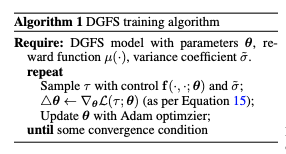
\includegraphics[width=0.9\textwidth]{figures/algo.png}
    \end{figure}

\end{frame}


%------------------------------------------------
\section{Diffusion Generative Flow Sampler Results}

\subsection{Gradients Variance Reduction and $Z$ estimation}

\begin{frame}[t]{Reduction of gradient variance}
\footnotesize

\begin{figure}
    \centering
    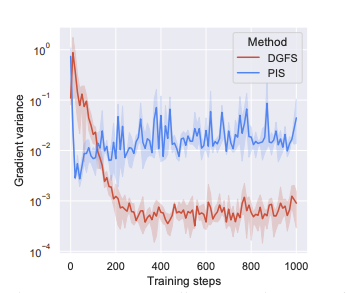
\includegraphics[width=0.4\textwidth]{figures/grad_variance.png}
    \caption{Gradient variance comparison between DGFS and PIS. DGFS shows significantly lower variance, leading to more stable training.}
\end{figure}

\end{frame}

\begin{frame}[t]{Accurate partition function $Z$ estimation}
\footnotesize

\textbf{Estimation of the partition function.} For an arbitrary trajectory $\tau = \{x_n\}_{n=0}^N$, one could define its (log) importance weight to be $S(\tau; \theta) = \log P(x_{0:N}) - \log Q(x_{0:N}; \theta)$, where $Q(x_{0:N}; \theta) = p^{\text{ref}}_0(x_0) \prod_{n=0}^{N-1} P_F(x_{n+1}|x_n; \theta)$.

\textbf{Log-partition function (log Z) estimator:}
\[
\log \sum_{b=1}^B \exp(S(\tau^{(b)}; \theta)) - \log B \leq \log Z, \quad \tau^{(b)} \sim Q(\cdot; \theta).
\]

\textbf{Explanation.}
\begin{itemize}\itemsep2pt
  \item $S(\tau; \theta)$: The log importance weight, measuring how much more likely the trajectory is under the target $P$ (which has terminal marginal $\pi \propto \mu$) than under the learned $Q$.
  \item $Q(x_{0:N}; \theta)$: The learned path measure, with terminal marginal approximating $\pi$.
  \item The estimator uses importance sampling: Sample trajectories from $Q$, compute their weights, and average in log space to estimate $\log Z$.
  \item The inequality $\leq \log Z$ holds because $Q$ approximates $P$, providing a lower bound on $\log Z$.
  \item This gives an accurate estimate of $Z$ without needing samples from $\pi$, leveraging the learned model.
\end{itemize}

\end{frame}

\begin{frame}[t]{Partition function estimation results}
\footnotesize

\begin{figure}
    \centering
    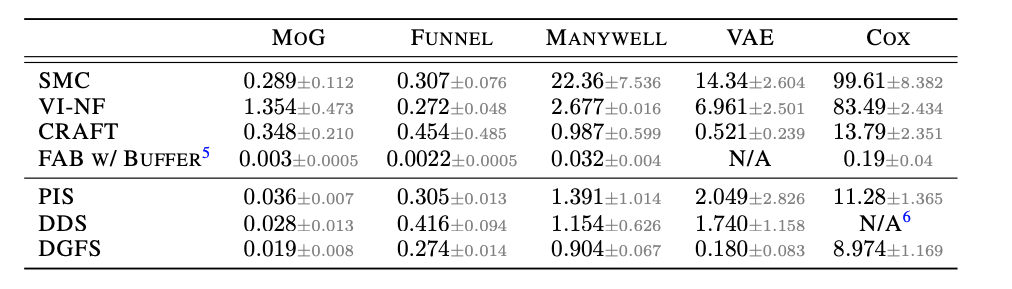
\includegraphics[width=1.025\textwidth]{figures/partition_fnct.png}
    \caption{To write a caption}
\end{figure}

\end{frame}

\begin{frame}[t]{Mode coverage results}

\begin{columns}[t]
\begin{column}{0.48\textwidth}
\begin{figure}
    \centering
    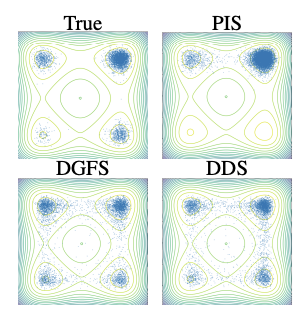
\includegraphics[width=0.5\textwidth]{figures/mode.png}
    \caption{Manywell plots. DGFS and DDS but not PIS recover all modes}
\end{figure}
\end{column}
\begin{column}{0.48\textwidth}
\begin{figure}
    \centering
    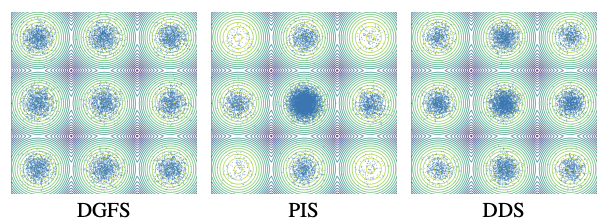
\includegraphics[width=0.9\textwidth]{figures/MoG.png}
    \caption{MoG visualization of DGFS and other diffusion-based samplers shows that DGFS could capture the diverse modes well. The contours display the landscape of the target density}
\end{figure}
\end{column}
\end{columns}
    
\end{frame}

\subsection{Convergence Guarantees}

\begin{frame}[t]{Convergence Theorem}
\footnotesize

\textbf{Convergence Guarantees for DGFS.}
\begin{itemize}\itemsep2pt
  \item Previous studies (Bortoli, 2022; Chen et al., 2022; Lee et al., 2022) show that the terminal sample distribution of a diffusion model converges to the target under mild assumptions if the control term is well learned. These apply to DGFS since proofs are independent of training method.
  \item Zhang et al. (2022a) prove that a perfectly learned score corresponds to zero GFlowNet training loss (Bengio et al., 2021; 2023), ensuring a well-trained DGFS accurately samples from the target distribution.
\end{itemize}

\end{frame}

\begin{frame}[t]{Off-policy training capability}
    \footnotesize

\end{frame}



%------------------------------------------------
\section{Conclusion}

\subsection{Summary}
\begin{frame}{Conclusion}
\footnotesize

\textbf{Summary of DGFS.} We propose the Diffusion Generative Flow Sampler (DGFS), a novel algorithm that trains diffusion models to sample from given unnormalized target densities. Different from prior works that could only learn from complete diffusion chains, DGFS can update its parameters with only partial specification of the stochastic process trajectory; moreover, DGFS can receive intermediate signals before completing the entire path. These features help DGFS benefit from efficient credit assignment and thus achieve better partition function estimation bias in the sampling benchmarks.

\end{frame}

\subsection{Q\&A}

\begin{frame}{Questions and hopefully answers :)}
    \centering
    \Huge Questions?
\end{frame}


\end{document}